\section{Dinámicas locales}

En la sección \ref{sec:Ch1PartialTrace} se habló de estados factorizables como aquellos estados que, descritos por un operador de densidad $\rho\in\densityspace{n}$, tienen la forma
\begin{equation}
    \rho=\rho_{A}\otimes\rho_{B},\nonumber
\end{equation}
donde $\rho_{A}\in\densityspace{m}$, $\rho_{B}\in\densityspace{l}$ y $l+m=n$. Siguiendo esta línea de pensamiento, con \textit{dinámicas factorizables} nos referimos a dinámicas unitarias generadas por hamiltonianos que no contienen un término de interacción (que en el caso de dos partículas son hamiltonianos de la forma $\mcH=H_{1}\otimes\Id+\Id\otimes H_{2}$), y que por lo mismo son descritas por operadores $\mcU\in\unitaryspace{n}$ \ddnote{cambié la notación del grupo unitario por la estándar (y correcta, si tienes dudas, me preguntas)} del tipo
\begin{equation}
    \mcU=U_{A}\otimes U_{B}.\nonumber
\end{equation}
De nuevo, $U_{A}\in\unitaryspace{m}$, $U_{B}\in\unitaryspace{l}$ y $l+m=n$. Los operadores locales están compuestos por operadores que actúan de forma independiente sobre diferentes subsistemas del sistema en cuestión. En el caso de un sistema compuesto por dos subsistemas de dos niveles, el operador local está compuesto por dos unitarias que actúan sobre $\hilbert_{2}$. Como el estado de máxima entropía resulta ser factorizable, las dinámicas locales son una muy buena primera forma de aplicar el formalismo descrito en las secciones anteriores.

Considérese la aplicación de grano grueso de $n$ a $1$ partículas definida según (\ref{eq:CG}), un estado efectivo $\rho_{\ef}\in\densityspace{2}$ y la aplicación de máxima entropía compatible dada por (\ref{eq:MaxEntAss}). Si la evolución microscópica es local entonces es generada por un hamiltoniano de la forma
\begin{equation}
    \mcH=\sum_{k=1}^{n}\omega_{k}\Id_{2^{k-1}}\otimes H_{k} \otimes \Id_{2^{n-k}},\nonumber
\end{equation}
siendo la unitaria 
\begin{equation}\label{eq:NFactorUnitaries}
    \mcU_{t}=\Motimes_{k=1}^{n}\text{exp}\qty(-\rmi\omega_{k}H_{k}t)=\Motimes_{k=1}^{n} U_{k}(t).
\end{equation}
A partir de este momento, para hacer más limpia la lectura de este documento se omitirán los productos tensoriales con operadores identidad. El subsistema sobre el que actúe un operador será denotado por un subíndice, de tal manera que el hamiltoniano previamente definido queda
\begin{equation}
    \mcH=\sum_{k=1}^{n}\omega_{k}H_{k}.\nonumber
\end{equation}


\subsection{Caso general}

Si se considera una evolución unitaria de la forma (\ref{eq:NFactorUnitaries}), y se propaga al estado obtenido de la aplicación de máxima entropía, el estado evolucionado es
\begin{equation}
    \varrho_{\max}(t)=\Motimes_{k=1}^{n}\frac{1}{Z_{k}}U_{k}(t) e^{\qty(p_{k}\sum_{j}\lambda_{j}\pauli{j})} (U_{k}(t))^{\dag}\nonumber
\end{equation}
El estado efectivo evolucionado en términos de los multiplicadores de Lagrange queda
\begin{equation}\label{eq:SeparableEvolution}
    \Gamma_{t}(\rho_{\ef})=\sum_{k=1}^{n}p_{k} U_{k}(t) \rho_{k} (U_{k}(t))^{\dag}.
\end{equation}
donde $\rho_{k}=\frac{1}{Z_{k}}e^{\qty(p_{k}\sum_{j}\lambda_{j}\pauli{j})}$. 

Por supuesto, esta expresión puede expandirse en términos de exponenciales o de funciones hiperbólicas del vector de Bloch del estado efectivo inicial, $\vec{r}_{\ef}$. Haciendo esto se obtiene una expresión para el valor esperado de $\pauli{j}$ a un tiempo $t$,
\begin{equation}\label{eq:SeparableEvolutionExpVal}
    \expval{\pauli{i}(t)}=\frac{1}{2}\sum_{k=1}^{n}p_{k}\tanh(p_{k}\lambda)\Tr[\pauli{j}U_{k}(t) (\hat{r}_{\ef}\cdot\vec{\sigma}) (U_{k}(t))^{\dag}]
\end{equation}
Si se piensa en el caso en que $p_{1}>p_{j}\,\forall j\neq 1$, separar la contribución del sistema de interés,
\begin{align}
    \expval{\pauli{j}(t)}=&\frac{1}{2}p_{1}\tanh(p_{1}\lambda)\Tr[\pauli{j}U_{1}(t) (\hat{r}_{\ef}\cdot\vec{\sigma}) (U_{1}(t))^{\dag}]\nonumber\\
    &+\frac{1}{2}\sum_{k=2}^{n}p_{k}\tanh(p_{k}\lambda)\Tr[\pauli{j}U_{k}(t) (\hat{r}_{\ef}\cdot\vec{\sigma}) (U_{k}(t))^{\dag}]\nonumber,
\end{align}
permite reconocer dos términos: uno asociado a la evolución \textit{sin error} de nuestro sistema, descrita por el operador unitario $U_{1}(t)$, y un término de ruido. La acción de este término dependerá tanto de la naturaleza de las evoluciones locales del entorno, como del número de partículas en este.


Por otro lado, en el caso en el que no hay partícula prioritaria, \ie ($p_{j}=\frac{1}{n}\forall j$), la relación entre la magnitud del vector de Bloch del estado efectivo y los multiplicadores de Lagrange es $\lambda=n\tanh^{-1}(r)$. Esto significa que la expresión del valor esperado de $\sigma_{j}$ a un tiempo $t$ es
\begin{equation}
    \expval{\pauli{j}(t)}=\frac{1}{2n}\sum_{k=1}^{n}\Tr[\pauli{j}U_{k}(t) (\vec{r}_{\ef}\cdot\vec{\sigma}) (U_{k}(t))^{\dag}],\nonumber
\end{equation}
que no es más que una combinación lineal de las mismas componentes evolucionadas de formas diferentes.
\subsection{Ejemplos particulares}

\subsubsection{Dinámica local simétrica}

Comenzamos con el caso en el que la dinámica local simétrica, esto es, de una unitaria $\mcU\in\unitaryspace{2^{n}}$ de la forma
\begin{equation}
    \mcU_{t}=\Motimes_{k=1}^{n}U(t),\nonumber
\end{equation}
donde $U(t)\in\unitaryspace{2}$. Se aplica la evolución al estado de máxima entropía compatible con un conjunto de observables tomográficamente completos en $\hilbert_{2}$ y se propaga al estado con la unitaria subyacente, para luego pasarlo por la aplicación de grano grueso y recuperar el estado efectivo evolucionado. Este caso es quizá el más sencillo, pues la simetría de la unitaria permite factorizarla:
\begin{align}
\mcC\qty[\Motimes_{k=1}^{n}U(t) \rho_{k} (U(t))^{\dag}]&=\sum_{k=1}^{n}p_{k} U(t) \rho_{k} (U(t))^{\dag}\nonumber \\
&=U(t)\qty(\sum_{k=1}^{n}p_{k} \rho_{k}) (U(t))^{\dag}\nonumber\\
&=U(t)\rho_{\ef}(U(t))^{\dag}.\nonumber
\end{align}
La dinámica efectiva tiene la forma
\begin{equation}\label{eq:EffectiveSymmetricLocal}
    \Gamma_{t}(\rho_{\ef})=U(t)\rho_{\ef}U^\dag(t).
\end{equation}\ddnote{embellecí un poco esta ecuación}
Este resultado es natural. No solo no hay interacción entre los diferentes subsistemas, significando esto que no se \textit{filtra} ningún tipo de información entre la partícula de interés y el resto, sino que cada parte evoluciona de manera idéntica: bajo la aplicación de grano grueso, lo que se observa es una combinación de $n$ entidades idénticas evolucionando de la misma forma.

\subsubsection{Particulas no preferenciales invariantes}

Centrémonos, momentáneamente, en el régimen de partícula preferencial, \ie{} $p_{1}>p_{j}\,\forall j\neq 1$. Asúmase que la probabilidad de detectar a la $k$-ésima partícula es la misma para todas excepto la primera. Entonces
\begin{equation}
    p_{k}=\frac{(1-p_{1})}{n-1}\text{ }\forall k\neq 1.\nonumber
\end{equation}
El estado de máxima entropía compatible con un estado efectivo $\rho_{\ef}$ es
\begin{equation}
    \varrho_{\max}=\rho_{1}\otimes\qty(\Motimes_{k=2}^{n}\frac{1}{Z_{k}}e^{\frac{(1-p_{1})}{n-1}\sum_{j}\lambda_{j}\pauli{j}}),\nonumber
\end{equation}
donde, para todo $k\neq 1$ se cumple que
\begin{equation}
    \frac{1}{Z_{k}}e^{\frac{1-p_{1}}{n-1}\sum_{j}\lambda_{j}\pauli{j}}=\frac{1}{2}\qty(\Id+\tanh(\frac{1-p_{1}}{n-1}\lambda)\hat{r}_{\rho}\cdot\vec{\sigma})\equiv \rho_{\text{np}}.\nonumber
\end{equation}
Como a cada partícula no preferencial se le asigna el mismo estado $\rho_{\text{np}}$, el estado del conjunto de partículas no preferenciales es
\begin{equation}
    \Motimes_{k=2}^{n}\rho_{k}=\rho_{\text{np}}^{\otimes(n-1)}\nonumber.
\end{equation}
Consíderese ahora la dinámica local generada por el hamiltoniano
\begin{equation}
    \mcH=\omega H_{1}.\nonumber
\end{equation}
Es decir, la dinámica en la que las partículas no preferenciales no varían, mientras que el subsistema de interés se propaga de forma unitaria. En este caso la dinámica efectiva es
\begin{equation}
    \Gamma_{t}(\rho_{\ef})=p_{1}U_{1}(t)\rho_{1}(U_{1}(t))^{\dag}+(1-p_{1})\rho_{\text{np}}.\nonumber
\end{equation}
En términos del vector de Bloch del estado efectivo inicial, con $r_{1}=\tanh(p_{1}\lambda)$, $r_{\text{np}}=\tanh((1-p_{1})\lambda)$, y $R$ la rotación generada por $U_{1}6p$:
\begin{equation}
    r_{\ef}\hat{r}_{\ef}\mapsto p_{1}r_{1}R\hat{r}_{\ef}+(1-p_{1})r_{\text{np}}\hat{r}_{\ef}.\nonumber
\end{equation}
Esta expresión parece no dar demasiada información: es simplemente la combinación lineal de dos vectores de Bloch, uno que ha sido rotado y otro al que no se le ha hecho nada, pero recordando que el vector de Bloch del estado efectivo inicial cumple $r=p_{1}r_{1}+(1-p_{1})r_{\text{np}}$, esta puede ser manipulada para ver que
\begin{equation}
    r_{\ef}\hat{r}_{\ef}\mapsto R(r_{\ef}\hat{r}_{\ef}-(1-p_{1})r_{\text{np}}\hat{r}_{\ef})+(1-p_{1})r_{\text{np}}\hat{r}_{\ef}.\nonumber
\end{equation}
El resultado es una rotación alrededor de una línea que no pasa por el origen. Una rotación de esta naturaleza puede descomponerse en una rotación a través de un eje que pasa por el origen $R_{0}$ y una traslación $T$ como $T^{-1}\circ R_{0}\circ T$. Nótese que una transformación así no tendría por qué mantener a los estados dentro de la esfera de Bloch, por lo que esta debe depender del estado mismo. \ddnote{Te felicito por esta observación}

\begin{figure}[ht!]
    \centering
    \begin{subfigure}{0.32\textwidth}
      \centering
      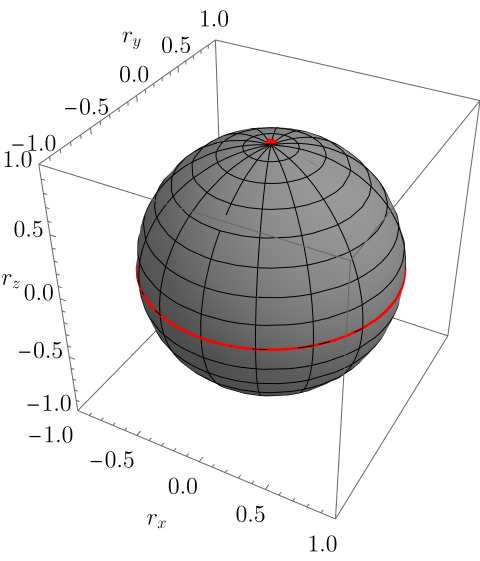
\includegraphics[width=0.9\linewidth]{chapter3/figures_separable/szxId_t=0._p=0.6_r=0.9.png}
      \caption{$t=0.0$}
    \end{subfigure}%
    \begin{subfigure}{0.32\textwidth}
      \centering
      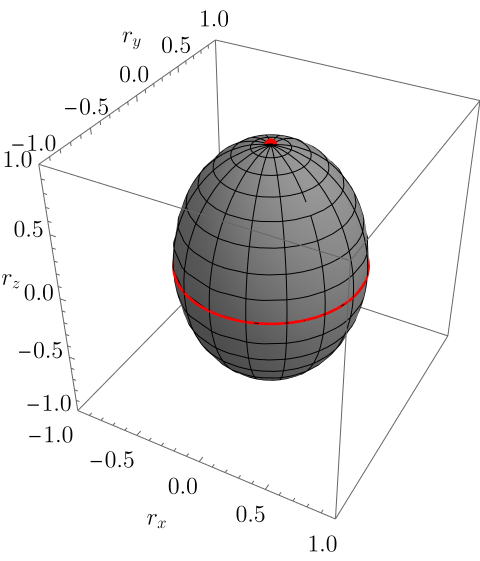
\includegraphics[width=0.9\linewidth]{chapter3/figures_separable/szxId_t=0.25_p=0.6_r=0.9.png}
      \caption{$t=0.25$}
    \end{subfigure}
    \begin{subfigure}{0.32\textwidth}
      \centering
      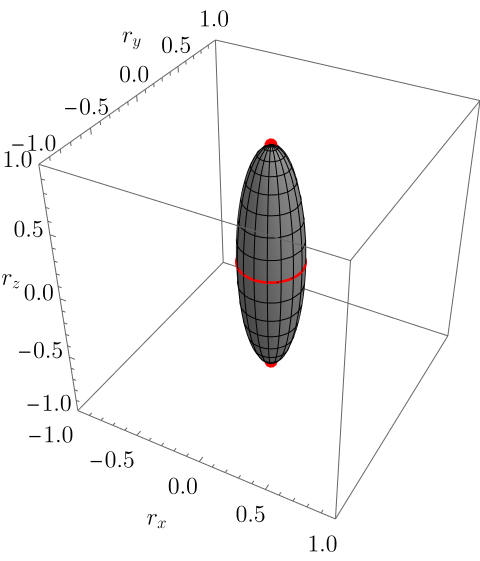
\includegraphics[width=0.9\linewidth]{chapter3/figures_separable/szxId_t=0.5_p=0.6_r=0.9.png}
      \caption{$t=0.5$}
    \end{subfigure}
    \caption{Efecto de la dinámica efectiva inducida por la unitaria microscópica $\mcU=U_{1}\otimes\Id_{2^{n-1}}$ sobre la esfera de Bloch cuando $r_{\ef}=0.9$, $p_{1}=0.6$ y $U_{1}=e^{-i\pi t \pauli{3}}$. La dramática contracción a lo largo de $r_{z}$ se asocia al alto valor de $1-p_{1}$. \label{fig:FaseChangeSequence}}
\end{figure}

En efecto, la traslación tiene una magnitud $(1-p_{1})r_{\text{np}}$ (a notar que la traslación es pequeña, y corresponde al término de ruido) en la dirección opuesta a la del estado (i.e. depende del estado tanto en magnitud como en dirección). Así que, aunque esto podría parecer una transformación afín, no lo es, pues depende enteramente del estado. Esto significa que la evolución efectiva no es lineal, y no tiene expresión en términos de operadores de Kraus. La figura \ref{fig:FaseChangeSequence} muestra el efecto que una dinámica de este estilo tiene sobre la esfera de Bloch (en particular, el caso $U_{1}=e^{-\rmi\omega t \pauli{3}}$). La contracción a lo largo del eje $r_{z}$ es un resultado del alto valor de $(1-p_{1})$ (0.4), y no sería visible si $p_{1}\rightarrow 1$.


En efecto, si $p_{1}\approx\frac{1}{2}$, entonces $\rho_{1}\approx\rho_{\ef}$, $\rho_{\text{np}}\approx\rho_{\ef}$, y la dinámica efectiva no solo sería lineal, sino que se convertiría en un canal de desfasamiento:

\begin{align}
    \Gamma_{t}(\rho_{\ef})=&p_{1}e^{-\rmi\omega t \pauli{3}}\rho_{1}e^{\rmi\omega t \pauli{3}}+(1-p_{1})\rho_{\text{np}}\nonumber\\
    \approx&\frac{1}{2}(\rho_{\ef}+e^{-\rmi\omega t \pauli{3}}\rho_{\ef} e^{\rmi\omega t \pauli{3}}),\nonumber
\end{align}
cuyos operadores de Kraus son $\frac{1}{\sqrt{2}}\left\{\Id, e^{\rmi\omega t \pauli{3}} \right\}$.
\subsubsection{Partícula preferencial invariante}

Ahora asumamos que es el sistema preferencial el que no evoluciona, mientras que las demás partículas sí lo hacen. Existen diferentes formas de abordar este problema, según la elección de las probabilidades y de la naturaleza de la evolución del resto de las partículas. Quizá el caso más sencillo es aquel en el que todas las partículas no preferenciales evolucionan de la misma forma. Esto es, una evolución generada por un hamiltoniano de la forma
\begin{equation}
    \mcH=\omega \sum_{k=2}^{n}H_{k}.\nonumber
\end{equation}
Sin perdida de generalidad, tómese $H_{k}=\pauli{3}\,\forall k$. Recordando la ecuación (\ref{eq:rhoArhoB}), los valores de expectación de $\pauli{j}$ serán
\begin{align}
    \expval{\pauli{1}(t)}=&p_{1} \expval{\sigma_{1}(0)}_{1}+\sum_{k=2}^{n}p_{k}\Tr[\pauli{1}e^{-\rmi\omega t\pauli{3}} \rho_{k} e^{\rmi\omega t\pauli{3}}]\nonumber\\
    \expval{\pauli{2}(t)}=&p_{1} \expval{\sigma_{2}(0)}_{1}+\sum_{k=2}^{n}p_{k}\Tr[\pauli{2}e^{-\rmi\omega t\pauli{3}} \rho_{k} e^{\rmi\omega t\pauli{3}}]\nonumber\\
    \expval{\pauli{3}(t)}=&\expval{\pauli{3}(0)}_{\ef},\nonumber
\end{align}
que quizá sea más clara escribiéndose en términos de las componentes de los vectores de Bloch de cada partícula (el primer subíndice indica la componente del vector, mientras que el segundo denota la partícula a la que pertenece):
\begin{align}
    r_{1,\ef}(t)=&r_{1,1}(0)+\sum_{k=2}^{n}p_{k}(r_{1,k}\cos(2\omega t)-r_{2,k}\sin(2\omega t))\nonumber\\
    r_{2,\ef}(t)=&r_{2,1}(0)+\sum_{k=2}^{n}p_{k}(r_{2,k}\cos(2\omega t)+r_{1,k}\sin(2\omega t))\nonumber\\
    r_{3,\ef}(t)=&r_{3,\ef}(0).\nonumber
\end{align}
Esto no es más que la aplicación de la misma rotación sobre todos los vectores de Bloch, a excepción del primero. Reescribiendo,
\begin{align}
    \vec{r}_{\ef}(t)=&p_{1}\vec{r}_{1}+R_{z}(2\omega t)\vec{r}_{e}\nonumber\\
    =&\vec{r}_{\ef}(0)+(R_{z}(2\omega t)-\Id)\vec{r}_{e}\nonumber
\end{align}
donde $\vec{r}_{e}\sum_{k=2}^{n}p_{k}\vec{r}_{k}$.
En este caso, el primer término es el término invariante, y sería lo único visible en el caso en que el aparato de medición no fallara, mientras que el segundo término corresponde a pequeñas oscilaciones completamente dependientes del estado efectivo inicial que nunca aumentan la pureza del estado. En efecto, considérese un estado efectivo inicial correspondiente a un sistema microscópico de $10$ qubits cuyo vector de Bloch tiene radio $r_{\ef}=0.95$ y tal que $p_{1}=0.99$ y $p_{j}=\frac{0.01}{9}\,\forall\,j\neq $. La magnitud del error absoluto, esto es, la distancia del estado efectivo evolucionado al estado efectivo inicial es
\begin{equation}
    \mcO_{t}=\norm{\vec{r}_{\ef}(0)-p_{1}\vec{r}_{1}-R_{z}(2\omega t)\vec{r}_{e}}=\norm{\vec{r}_{e}-R_{z}(2\omega t)\vec{r}_{e}}\nonumber.
\end{equation}
Ahora, esta magnitud es máxima cuando $t=\frac{\pi}{2\omega}$, pero depende también de las componentes de $\vec{r}_{ef}$. Por simplicidad, asumamos que el estado efectivo inicial no tiene componente en $z$. Entonces
\begin{equation}
    \mcO_{\max}=\norm{-2\vec{r}_{e}}=1.08\times 10^{-3}\nonumber.
\end{equation}
Estas pequeñas oscilaciones son, justamente, el término de ruido. La visualización a la solución del problema puede observarse en la Figura \ref{fig:OscilationsSameHam}. Cada una de las componentes del vector de Bloch efectivo se ve como una suma de una constante con funciones periódicas que tienen el mismo periodo, o  como la suma de una constante más una función periódica (viendo la combinación de los vectores de cada partícula no preferencial como una partícula efectiva). De cualquier forma, el resultado es una función periódica.

\begin{figure}[ht!]
    \centering
    \begin{subfigure}{0.5\textwidth}
      \centering
      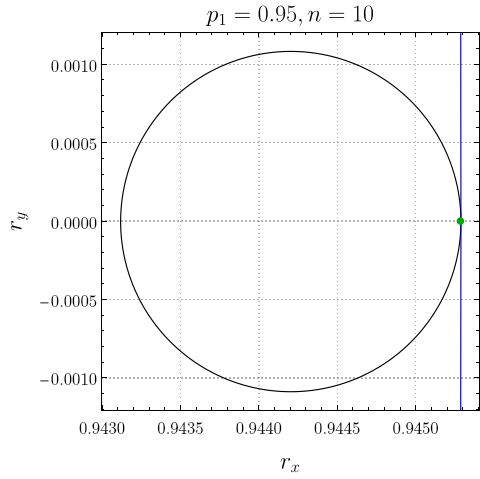
\includegraphics[width=0.9\linewidth]{chapter3/figures_separable/local_prefinv_eq_n=10_p=0.95.png}
    \end{subfigure}%
    \begin{subfigure}{0.5\textwidth}
      \centering
      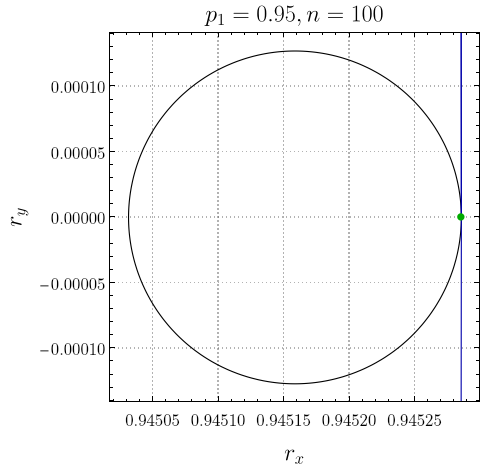
\includegraphics[width=0.9\linewidth]{chapter3/figures_separable/local_prefinv_eq_n=100_p=0.95.png}
    \end{subfigure}
    \caption{Oscilaciones periódicas correspondientes a la dinámica efectiva inducida por el hamiltoniano microscópico $\mcH=\omega\sum_{k=2}^{n}\pauli{3,k}$ en un sistema de $n$ partículas. En azul, el conjunto de estados con el mismo radio de Bloch ($r_{\ef}=0.95$) y el mismo $r_{z}$ (aprox. $0.09$) que el estado efectivo inicial (en verde). \label{fig:OscilationsSameHam}}
\end{figure}

Si, por otro lado, quitamos la restricción de que todas las partículas no preferenciales evolucionen con la misma frecuencia, se vuelve imposible factorizar la rotación:
\begin{equation}
    \vec{r}_{\ef}(t)=p_{1}\vec{r}_{1}+\sum_{k=2}^{n} p_{k}R_{z}(2\omega_{k} t)\vec{r}_{k}.\nonumber
\end{equation}
Ahora cada partícula no preferencial contribuye al error de forma única, y a pesar de que la evolución de cada partícula no preferencial sea periódica, la combinación de estas no tiene por qué serlo. El resultado ahora depende de las frecuencias de evolución de cada partícula, de sus pesos $p_{k}$, y del número $n$ de partículas en el sistema microscópico (si $n=2$ se recupera el caso anterior). Las componentes del vector de Bloch del estado efectivo evolucionado,
\begin{align}
    r_{1,\ef}(t)=&r_{1,1}(0)+\sum_{k=2}^{n}p_{k}(r_{1,k}\cos(2\omega_{k} t)-r_{2,k}\sin(2\omega_{k} t))\nonumber\\
    r_{2,\ef}(t)=&r_{2,1}(0)+\sum_{k=2}^{n}p_{k}(r_{2,k}\cos(2\omega_{k} t)+r_{1,k}\sin(2\omega_{k} t))\nonumber\\
    r_{3,\ef}(t)=&r_{3,\ef}(0).\nonumber
\end{align}
revelan la complejidad de la evolución, además de su no-linealidad, pues los vectores $\vec{r}_{k}$ dependen del estado efectivo inicial a través del multiplicador de Lagrange $\lambda.$ Las figuras \ref{fig:PrefInv1} y \ref{fig:PrefInv2} muestran algunos ejemplos de la geometría de estas dinámicas, en las que las frecuencias $\omega_{k}$ se obtuvieron de una distribución uniforme $\text{U}[-3,3]$.

\begin{figure}[ht!]
    \centering
    \begin{subfigure}{0.5\textwidth}
      \centering
      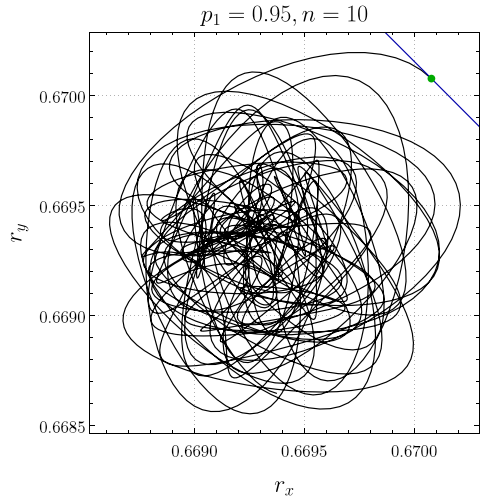
\includegraphics[width=0.9\linewidth]{chapter3/figures_separable/local_prefinv_ran_n=10_p=0.95_r=0.95_a=-3_b=3.png}
    \end{subfigure}%
    \begin{subfigure}{0.5\textwidth}
      \centering
      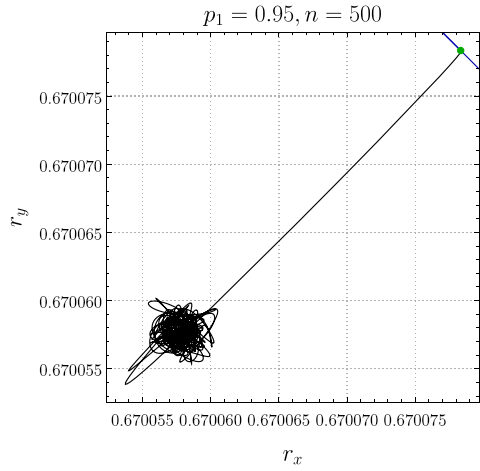
\includegraphics[width=0.9\linewidth]{chapter3/figures_separable/local_prefinv_ran_n=500_p=0.95_r=0.95_a=-3_b=3.png}
    \end{subfigure}
    \caption{Variaciones correspondientes a la dinámica efectiva inducida por el hamiltoniano $\mcH=\sum_{k=2}^{n}\omega_{k}\pauli{3,k}$ en un sistema de $n$ partículas. En azul, el conjunto de estados con el mismo radio de Bloch ($r_{\ef}=0.95$) y el mismo $r_{z}$ (aprox. $0.07$) que el estado efectivo inicial (verde). Valores de $p_{1}$ cercanos a $1$ conducen a variaciones menos importantes. \label{fig:PrefInv1}}
\end{figure}

\begin{figure}[ht!]
    \centering
    \begin{subfigure}{0.5\textwidth}
      \centering
      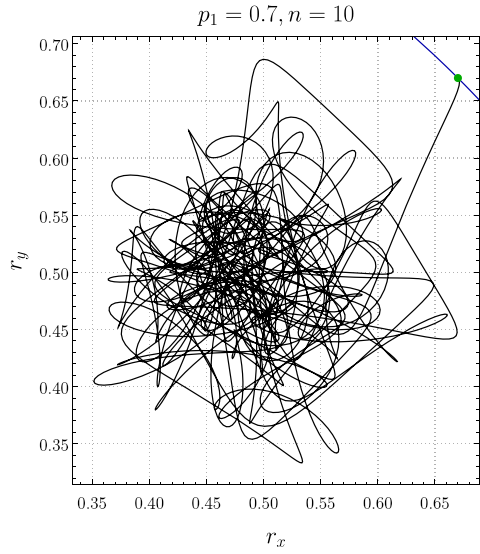
\includegraphics[width=0.9\linewidth]{chapter3/figures_separable/local_prefinv_ran_n=10_p=0.7_r=0.95_a=-3_b=3.png}
    \end{subfigure}%
    \begin{subfigure}{0.5\textwidth}
      \centering
      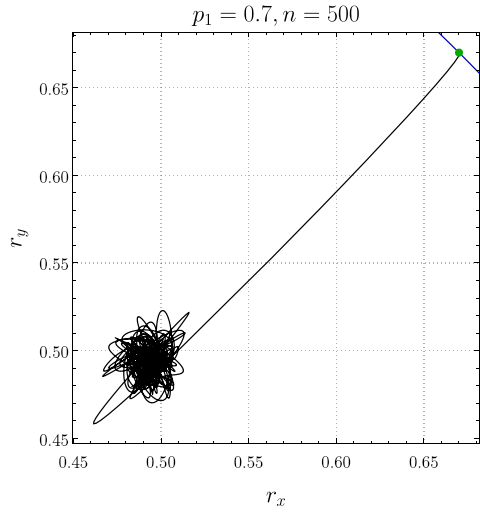
\includegraphics[width=0.9\linewidth]{chapter3/figures_separable/local_prefinv_ran_n=500_p=0.7_r=0.95_a=-3_b=3.png}
    \end{subfigure}
    \caption{Variaciones correspondientes a la dinámica efectiva inducida por el hamiltoniano $\mcH=\sum_{k=2}^{n}\omega_{k}\pauli{3,k}$ en un sistema de $n$ partículas. En azul, el conjunto de estados con el mismo radio de Bloch ($r_{\ef}=0.95$) y el mismo $r_{z}$ (aprox. $0.07$) que el estado efectivo inicial (verde). Valores de $p_{1}$ menores conducen a variaciones más importantes. \label{fig:PrefInv2}}
\end{figure}

\subsubsection{Partículas no interactuantes con diferente frecuencia de transición}

En los dos casos anteriores se permitió que alguna de las partes del sistema se mantuviera invariante, fuera la partícula preferencial o el resto. Veamos ahora qué sucede cuando se permite que todo el sistema evolucione. Considérese un hamiltoniano
\begin{equation}
    \mcH=\sum_{k=1}^{n}\omega_{k}\pauli{3,k},\nonumber
\end{equation}
de tal forma que toda la evolución mantenga constante la componente en $\pauli{3}$. Explícitamente, las componentes del vector de Bloch del estado efectivo siguen las ecuaciones
\begin{align}
    r_{1,\ef}(t)=&r_{1,1}(t)-\sum_{k=2}^{n}p_{k}A_{k}\sin(2\omega_{k} t-\phi_{k})\nonumber\\
    r_{2,\ef}(t)=&r_{2,1}(t)+\sum_{k=2}^{n}p_{k}A_{k}\sin(2\omega_{k} t+\theta_{k}),\nonumber
\end{align}
donde se omite la tercera componente, que no cambia, y
\begin{align}
    A_{k}=\sqrt{r_{1,k}^{2}+r_{2,k}^{2}} & & \phi=_{k}\arccos\qty(\frac{r_{2,k}}{\sqrt{r_{1,k}^{2}+r_{2,k}^{2}}}) & & \theta_{k}=\arcsin\qty(\frac{r_{1,k}}{\sqrt{r_{1,k}^{2}+r_{2,k}^{2}}})\nonumber
\end{align}
El comportamiento de los términos de suma depende de las frecuencias $\omega_{k}$, pero la amplitud de estas funciones oscilatorias puede acercarse arbitrariamente a $\sum_{k=2}^{n} p_{k} A_{k}$. Esto no significa que el error explote. En realidad, como $0\leq A_{k}\leq 1\,\forall k$, entonces $0\leq\sum_{k=2}^{n} p_{k} A_{k}\leq 1$. 


Para obtener resultados más específicos, asumamos que $p_{j}=p_{\text{np}}=\frac{1-p_{1}}{1-n}\,\forall\,j\neq 1$ y que $r_{3,\ef}=0$. Por construcción del estado de máxima entropía compatible con $\rho_{\ef}$,
\begin{align}
    r_{k}=r_{\text{np}}=\tanh(p_{\text{np}} \lambda) & & r_{j,k}=r_{\text{np}}\frac{r_{j,\ef}}{r_{\ef}}\nonumber
\end{align}
Esto significa que las expresiones previas se simplifican considerablemente, en efecto, las primeras dos componentes del vector pasan a ser
\begin{align}
    r_{1,\ef}(t)&=r_{1,1}(t)-p_{\text{np}}r_{\text{np}}\sum_{k=2}^{n}\sin(2\omega_{k} t-\phi)\nonumber\\
    r_{2,\ef}(t)&=r_{2,1}(t)+p_{\text{np}}r_{\text{np}}\sum_{k=2}^{n}\sin(2\omega_{k} t+\theta)\nonumber
\end{align}
Aquí pasa a ser claro que la amplitud máxima de la oscilación de error de cada componente es $(1-p_{1})r_{\text{np}}$, que en el caso en que $r_{\ef}=0.9$, $p=0.95$ y $n=100$ es $4.79\times 10^{-5}$, pero si $p_{1}=0.5$ es $0.4$. Las figuras \ref{fig:Oscilations12} y \ref{fig:Oscilations13} muestran algunos ejemplos de este tipo de dinámica.

\begin{figure}[ht!]
    \centering
    \begin{subfigure}{0.5\textwidth}
      \centering
      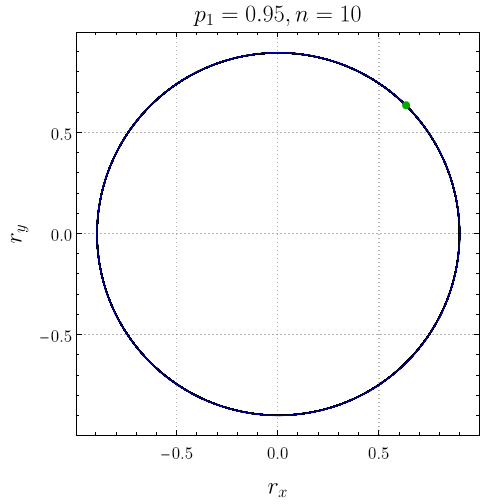
\includegraphics[width=0.9\linewidth]{chapter3/figures_separable/local_all_ran_p=0.95_r=0.9_n=10_a=-3_b=3.png}
    \end{subfigure}%
    \begin{subfigure}{0.5\textwidth}
      \centering
      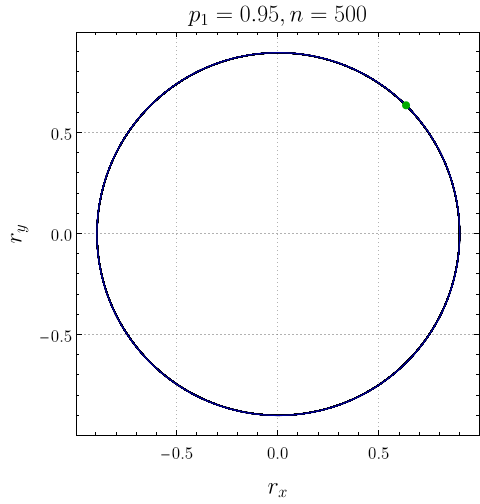
\includegraphics[width=0.9\linewidth]{chapter3/figures_separable/local_all_ran_p=0.95_r=0.9_n=500_a=-3_b=3.png}
    \end{subfigure}
    \caption{Variaciones correspondientes a la dinámica efectiva inducida por el hamiltoniano $\mcH=\sum_{k=1}^{n}\omega_{k}\pauli{3,k}$ en un sistema de $n$ partículas. Si $r_{\ef}=0.9$ y $p=0.95$ las variaciones debidas al error no son perceptibles debido a su pequeña amplitud. En verde, el estado efectivo inicial. En azul, la evolución del vector de Bloch que seguiría el sistema si $p_{1}=1$. \label{fig:Oscilations12}}
\end{figure}
\begin{figure}[ht!]
    \centering
    \begin{subfigure}{0.5\textwidth}
      \centering
      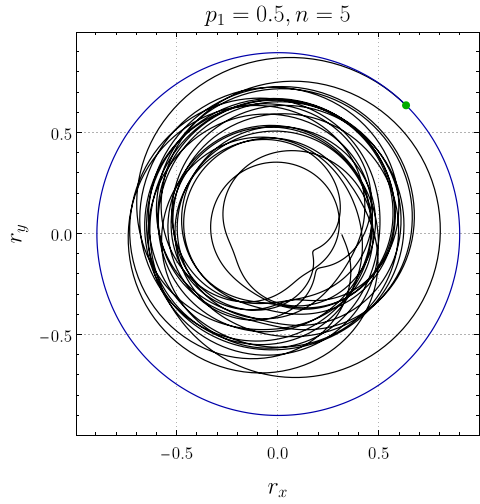
\includegraphics[width=0.9\linewidth]{chapter3/figures_separable/local_all_ran_p=0.5_r=0.9_n=5_a=-3_b=3.png}
    \end{subfigure}%
    \begin{subfigure}{0.5\textwidth}
      \centering
      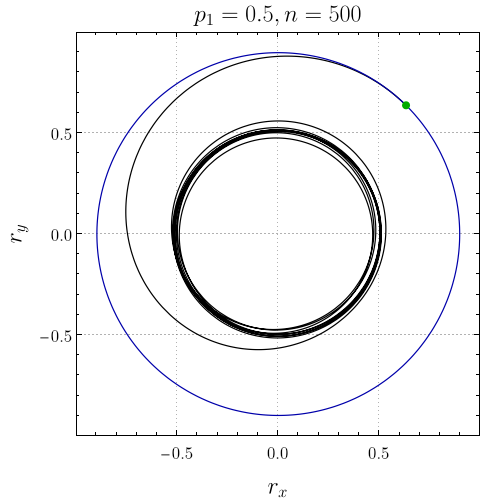
\includegraphics[width=0.9\linewidth]{chapter3/figures_separable/local_all_ran_p=0.5_r=0.9_n=500_a=-3_b=3.png}
    \end{subfigure}
    \caption{Variaciones correspondientes a la dinámica efectiva inducida por el hamiltoniano $\mcH=\sum_{k=1}^{n}\omega_{k}\pauli{3,k}$ en un sistema de $n$ partículas. Si $r_{\ef}=0.9$ y $p=0.5$ el alejamiento de la evolución esperada se hace notar. En verde, el estado efectivo inicial. Para valores grandes de $n$ se vuelve dominante el término de $p_{1}$. En azul, la evolución del vector de Bloch que seguiría el sistema si $p_{1}=1$. \label{fig:Oscilations13}}
\end{figure}

\newpage

\pagebreak